\documentclass[12pt, a4paper, oneside]{article}
\usepackage{amsmath, amsthm, amssymb, graphicx}
\usepackage[bookmarks=true, colorlinks, citecolor=blue, linkcolor=black]{hyperref}
\usepackage[margin = 25mm]{geometry}
\usepackage{setspace}
\usepackage{listings}
\usepackage{cite}
\usepackage{ctex}
\usepackage{tabularx}
\usepackage{fancyhdr}
\title{Homework 0:Nobel Laureates Related to Lasers}
\date{\today}
\author{物理2001孙陶庵202011010101\\https://github.com/xingxia1/test1}
\begin{document}
\begin{spacing}{2.0}
\maketitle


\section{Nobel prizes in Physics}


These are the Nobel prizes in Physics related to laser.\\
1.1964,for fundamental work in the field of quantum electronics, which has led to the construction of oscillators and amplifiers based on the maser-laser principle was awarded to Charles Hard Townes and Nicolay Gennadiyevich Basov and Aleksandr Mikhailovich Prokhorov.\\
Reason:pioneering studies of the laser.\\
2.1981, for their contribution to the development of laser spectroscopy\cite{RN12} was awarded to Nicolaas Bloembergen and Arthur Leonard Schawlow and Kai M. Siegbahn.\\
3.1997, for development of methods to cool and trap atoms with laser light\cite{RN11} was awarded to Steven Chu, Claude Cohen-Tannoudji and William D. Phillips\\
Reason:They used laser light to cool gases to the $\mu K$ temperature range and keeping the chilled atoms floating or captured in different kinds of “atom traps”.\\
This work increasing people knowledge of the interplay between radiation and matter. In particular, they give us a deeper understanding of the quantum physical behavior of cryogenic gases.\\
4.2002, for pioneering contributions to astrophysics, in particular for the detection of cosmic neutrinos" and the other half to Riccardo Giacconi\cite{RN09} was awarded to Raymond Davis Jr. and Masatoshi Koshiba\\
Reason:Riccardo Giacconi first successfully used X-ray (one of the laser) to detect the outside our solar system, and first to prove that the universe contains background radiation of X-ray light, also, detect most astronomers now consider to contain black holes. \\
5.2006, for their discovery of the blackbody form and anisotropy of the cosmic microwave background radiation\cite{RN06} was awarded to John C. Mather and George F. Smoot\\
Reason:Used the Cosmic Background Explorer (COBE)which involves DIRBE\cite{RN07} and FIRAS\cite{RN08} to discover the blackbody form and anisotropy of the cosmic microwave background radiation\\
6.2017, for decisive contributions to the LIGO detector and the observation of gravitational waves\cite{RN05} was awarded to Rainer Weiss, Barry C. Barish and Kip S. Thorne\\
Reason:"LIGO, the Laser Interferometer Gravitational-Wave Observatory", and laureates used this observatory to observe the gravitational wave for four decades.\\
\begin{figure}[htbp]
    \centering
    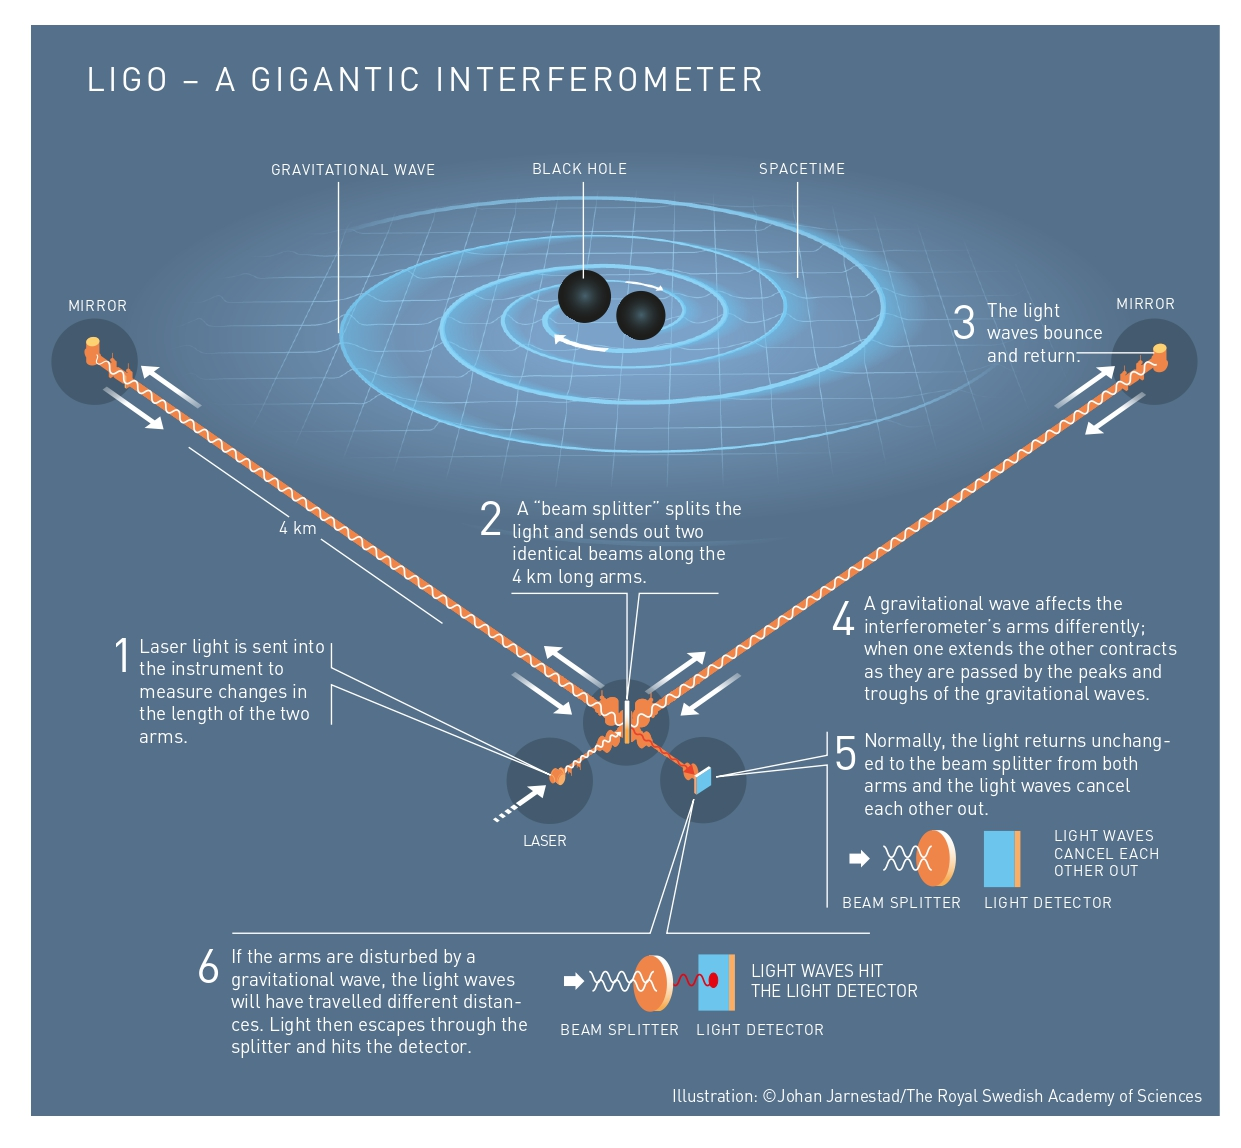
\includegraphics[width=8cm]{fig_fy_en_17_LIGO_page-0001.jpg}
    \caption{LIGO – A GIGANTIC INTERFEROMETER}
\end{figure}\\
7.2018, for groundbreaking inventions in the field of laser physics\cite{RN04} was awarded to Arthur Ashkin, Gérard Mourou and Donna Strickland\\
Reason:invented optical tweezers that grab particles, atoms, viruses and other living cells with their laser beam fingers.\cite{RN03}\\


\section{Nobel prizes in Chemistry}
These are the Nobel prizes in Chemistry related to laser.\\
1.1964,for her determinations by X-ray techniques of the structures of important biochemical substances\cite{RN14} was awarded to Dorothy Crowfoot Hodgkin.
Reason:Biochemical Analysis Experiments Using X-rays.\cite{HodgkinDorothy1937Xrca}
2.1999,for his studies of the transition states of chemical reactions using femtosecond spectroscopy
Reason:Used to demonstrate that using fast laser technology it is possible to observe how atoms in molecules move during chemical reactions.
\end{spacing}{}

\bibliographystyle{IEEEtran}
\bibliography{lecktion0}

\end{document}